\documentclass[11pt, a4paper]{article} % setsfont size and layout

%% required packages %%

\usepackage[margin=2.5cm]{geometry} % margins
\usepackage[utf8]{inputenc} % Umlaute
\usepackage{amsmath,amssymb, physics}		% math formulas
\usepackage{graphicx}		% graphics
\usepackage{fancyhdr}		% header and footer on every page
\usepackage{setspace}		% line space (e.g. \singlespacing, \onehalfspacing or \doublespacing)

\usepackage{braket}
\usepackage{xcolor}
%% Here the main part of the document begins %%

\begin{document}

%% Some more settings %%

\setlength{\parindent}{0pt} % first line in paragraph will not be indented
\onehalfspacing				% 1.5 line spacing
%\thispagestyle{empty}		% no header and page number on first page


%% Header on first page with course information etc. %
%\begin{tabular}{p{15.5cm}}
%	{\large \textbf{Classical Mechanics}} \\
%	Westlake University \\
%	\hline
%	\\
%\end{tabular}

\vspace*{0.1cm}				% vertical space between header on top of the page and main heading


\begin{center}
	{\Large \textbf{Classical Mechanics}}
    \vspace*{2mm}

    {\Large \textbf{Final Exam with Answer Key}}
	\vspace{8mm}
%Name:
%\end{center}
%\vspace{0.1cm}

{\Large \textbf{Time: 2:00--4:00 pm, Jan. 5th, 2026}}
\vspace*{2mm}

{\Large \textbf{Duration: 120 minutes}}
\vspace*{2mm}

{\Large \textbf{Total Points: 100 out of 108}}
\end{center}
\vspace*{8mm}

{\Large \textbf{Instruction:}}
\vspace*{2mm}

{\Large \textbf{This is a closed-book exam; no aids are allowed.}}
\vspace*{2mm}

{\Large \textbf{Total 11 pages including the front page of the instruction.}}
\vspace*{2mm}

{\Large \textbf{Provide relevant mathematical steps.}}
\vspace*{2mm}

{\Large \textbf{All answers must be in English.}}
\vspace*{2mm}

{\Large \textbf{Don't open the booklet before the exam begins.}}
\vspace{5cm}

\begin{center}
{\Large \textbf{Student Name:} \underline{\hspace{4cm}}}
\vspace*{8mm}

{\Large \textbf{Student ID:} \underline{\hspace{4cm}}}
\vspace*{2mm}
\end{center}

\newpage
\section*{Problem 1 [$5 + 5$ points]}
\begin{enumerate}
  \item[(1)] Write down Newton's second law, the Euler--Lagrange equation, and Hamilton's equations of motion.

  \item[(2)] Derive the Euler--Lagrange equation from Hamilton's principle. For a system with action
  \[
  S[q]=\int_{t_1}^{t_2} L(q,\dot{q},t)\,dt,
  \]
  show that the condition $\delta S=0$ for fixed-endpoint variations $\delta q(t_1)=\delta q(t_2)=0$ leads to the Euler--Lagrange equation.

\end{enumerate}

\subsection*{Solution}
\begin{enumerate}
\item[(1)] Newton's second law is
\[
\mathbf F=m\mathbf a.
\]

The Euler--Lagrange equation is
\[
\frac{d}{dt}\frac{\partial L}{\partial \dot q_i}
-
\frac{\partial L}{\partial q_i}
=0.
\]

Hamilton's equations are
\[
\dot q_i=\frac{\partial H}{\partial p_i},
\qquad
\dot p_i=-\frac{\partial H}{\partial q_i}.
\]

\item[(2)] Hamilton's principle states that the physical path satisfies
\[
\delta S=0,
\qquad
S[q]=\int_{t_1}^{t_2}L(q,\dot q,t)\,dt.
\]

The variation of the action is
\[
\delta S
=
\int_{t_1}^{t_2}
\left(
\frac{\partial L}{\partial q}\delta q
+
\frac{\partial L}{\partial \dot q}\delta \dot q
\right)dt.
\]

Since
\[
\delta \dot q=\frac{d}{dt}\delta q,
\]
we integrate the second term by parts:
\[
\int_{t_1}^{t_2}
\frac{\partial L}{\partial \dot q}\delta \dot q\,dt
=
\left[
\frac{\partial L}{\partial \dot q}\delta q
\right]_{t_1}^{t_2}
-
\int_{t_1}^{t_2}
\frac{d}{dt}\left(\frac{\partial L}{\partial \dot q}\right)
\delta q\,dt.
\]

For fixed endpoint variations,
\[
\delta q(t_1)=\delta q(t_2)=0,
\]
so the boundary term vanishes. Therefore
\[
\delta S
=
\int_{t_1}^{t_2}
\left[
\frac{\partial L}{\partial q}
-
\frac{d}{dt}\left(\frac{\partial L}{\partial \dot q}\right)
\right]\delta q\,dt.
\]

Since \(\delta q(t)\) is arbitrary,
\[
\boxed{
\frac{d}{dt}\frac{\partial L}{\partial \dot q}
-
\frac{\partial L}{\partial q}
=0.
}
\]

\end{enumerate}


\newpage
\section*{Problem 2 [$10$ points]}
Use the generating function $F_1(q,Q)=\frac{1}{2}m\omega q^2\cot Q$ for the harmonic oscillator with Hamiltonian $H(q,p)=\frac{p^2}{2m}+\frac{1}{2}m\omega^2q^2$ to find the transformed Hamiltonian $K(Q,P)$.

\subsection*{Solution}
The generating function is
\[
F_1(q,Q)=\frac12 m\omega q^2\cot Q.
\]

For an \(F_1(q,Q)\) generating function,
\[
p=\frac{\partial F_1}{\partial q},
\qquad
P=-\frac{\partial F_1}{\partial Q}.
\]

Therefore
\[
p=m\omega q\cot Q,
\]
and
\[
P=-\frac{\partial}{\partial Q}
\left(
\frac12 m\omega q^2\cot Q
\right)
=
\frac12 m\omega q^2\csc^2 Q.
\]

Thus
\[
q^2=\frac{2P}{m\omega}\sin^2 Q.
\]

Also,
\[
p^2=m^2\omega^2q^2\cot^2 Q.
\]

The transformed Hamiltonian is
\[
K(Q,P)=H(q,p).
\]

Since \(F_1\) has no explicit time dependence,
\[
K=H.
\]

Now
\[
H
=
\frac{p^2}{2m}
+
\frac12 m\omega^2q^2.
\]

Substituting \(p=m\omega q\cot Q\),
\[
H
=
\frac12 m\omega^2q^2\cot^2 Q
+
\frac12 m\omega^2q^2
=
\frac12 m\omega^2q^2(\cot^2 Q+1).
\]

Using
\[
\cot^2 Q+1=\csc^2 Q,
\]
we get
\[
H
=
\frac12 m\omega^2q^2\csc^2 Q.
\]

But
\[
P=\frac12 m\omega q^2\csc^2 Q.
\]

Therefore
\[
\boxed{
K(Q,P)=\omega P.
}
\]


\newpage
\section*{Problem 3 [$10$ points]}
A bead of mass $m$ slides without friction on a circular hoop of radius $R$. The hoop lies in a vertical plane, but is rotated about its vertical diameter. Suppose the angular velocity $\Omega(t)$ of the hoop is rapidly modulated in time: $\Omega(t)=\Omega_0+\epsilon \cos(\omega t),$ where $\epsilon \ll \omega$, but $\omega$ is very large compared with the natural gravitational frequency $\sqrt{g/R}$. Let $\theta$ be the angle of the bead measured from the top of the hoop, so that $\theta=0$ corresponds to the bead being at the unstable upper point when the hoop is not rotating. Using the Lagrangian formalism, derive the equation of motion for $\theta(t)$. Within small angle approximation, discuss qualitatively how the rapid modulation of $\Omega(t)$ can modify the stability of the top equilibrium.

\begin{figure}[h]
    \centering
    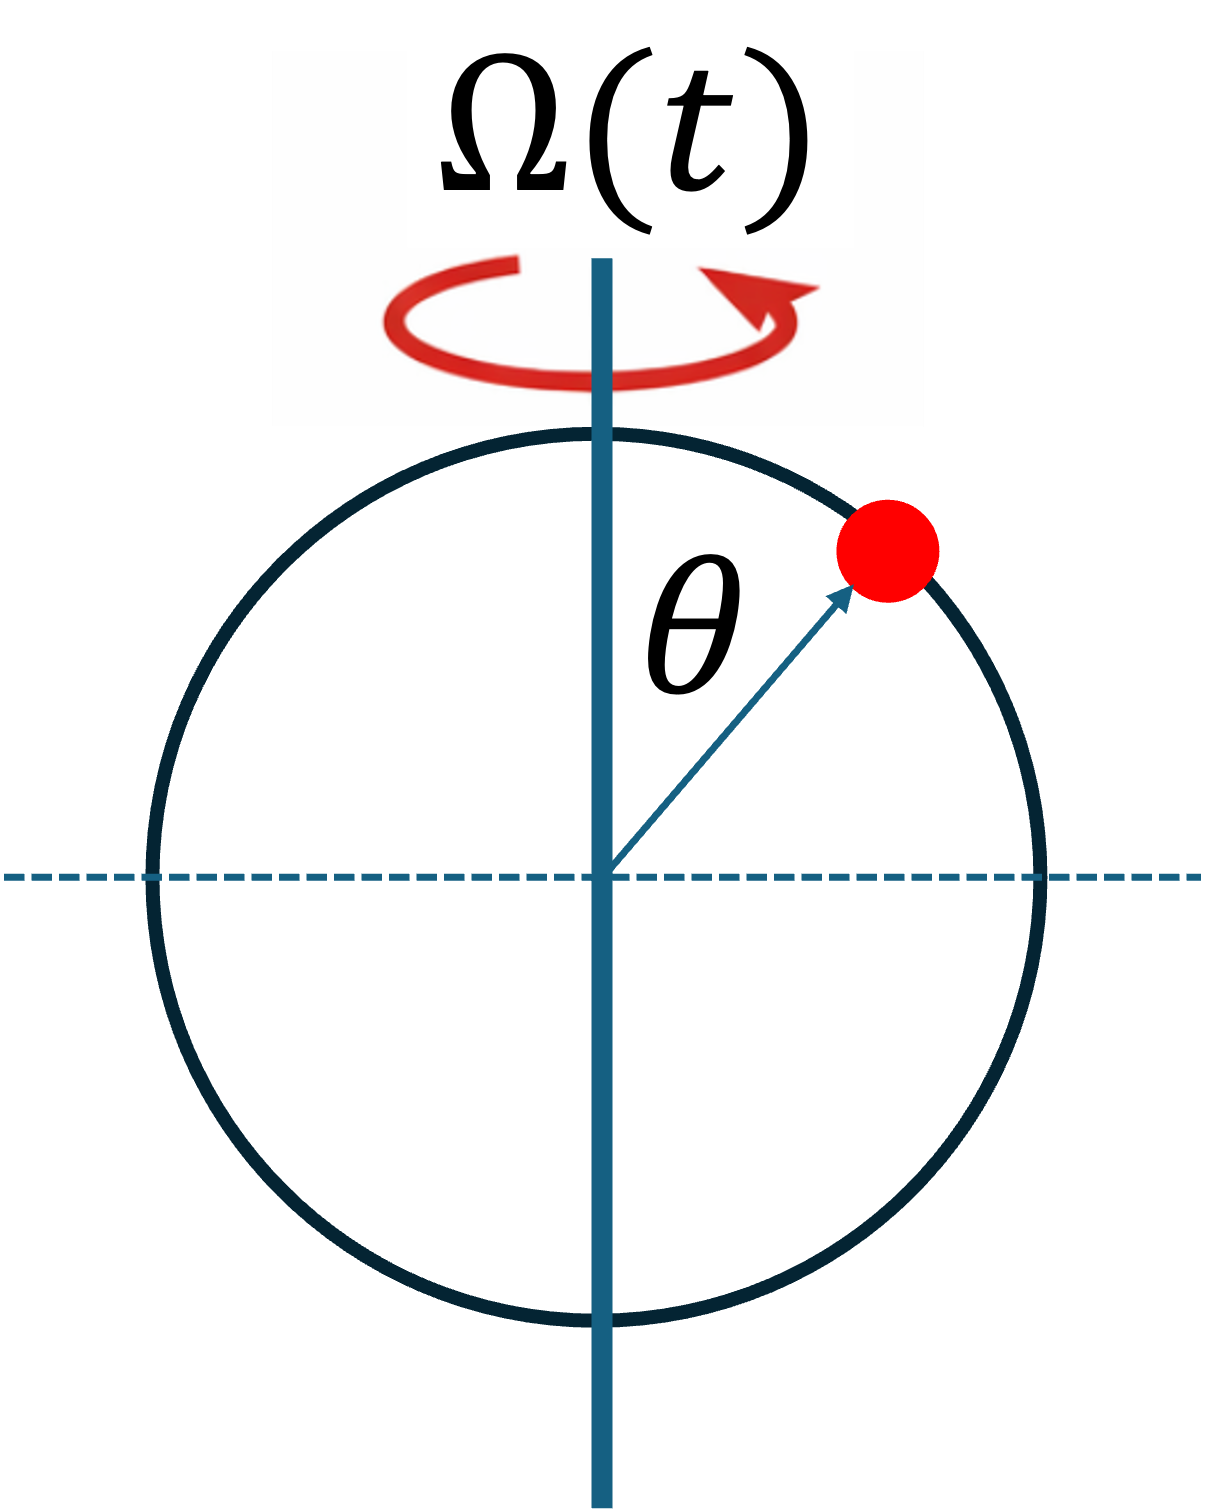
\includegraphics[width=0.3\textwidth]{P3.png}
    \label{P3}
\end{figure}

\subsection*{Solution}
Let \(\theta\) be measured from the top of the hoop. The bead has height
\[
z=R\cos\theta
\]
and distance from the vertical rotation axis
\[
\rho=R\sin\theta.
\]

The kinetic energy has two parts:
\[
T=\frac12 mR^2\dot\theta^2
+
\frac12 mR^2\Omega(t)^2\sin^2\theta.
\]

The gravitational potential energy is
\[
V=mgR\cos\theta.
\]

Thus
\[
L
=
\frac12 mR^2\dot\theta^2
+
\frac12 mR^2\Omega(t)^2\sin^2\theta
-
mgR\cos\theta.
\]

The Euler--Lagrange equation gives
\[
\frac{d}{dt}\left(mR^2\dot\theta\right)
-
\left[
mR^2\Omega(t)^2\sin\theta\cos\theta
+
mgR\sin\theta
\right]
=0.
\]

Therefore
\[
mR^2\ddot\theta
=
mR^2\Omega(t)^2\sin\theta\cos\theta
+
mgR\sin\theta.
\]

So
\[
\boxed{
\ddot\theta
=
\Omega(t)^2\sin\theta\cos\theta
+
\frac{g}{R}\sin\theta.
}
\]

With
\[
\Omega(t)=\Omega_0+\epsilon\cos(\omega t),
\]
the equation is
\[
\boxed{
\ddot\theta
=
\left[\Omega_0+\epsilon\cos(\omega t)\right]^2
\sin\theta\cos\theta
+
\frac{g}{R}\sin\theta.
}
\]

For small \(\theta\),
\[
\sin\theta\approx \theta,
\qquad
\cos\theta\approx 1,
\]
so
\[
\boxed{
\ddot\theta
\approx
\left[
\frac{g}{R}
+
\left(\Omega_0+\epsilon\cos(\omega t)\right)^2
\right]\theta.
}
\]

To first order in \(\epsilon\),
\[
\boxed{
\ddot\theta
\approx
\left(
\frac{g}{R}
+\Omega_0^2
+2\Omega_0\epsilon\cos\omega t
\right)\theta.
}
\]
Define
\[
a(t)=
\frac{g}{R}
+\Omega_0^2
+2\Omega_0\epsilon\cos(\omega t).
\]
The smallest possible value of this coefficient is
\[
a_{\min}
=
\frac{g}{R}
+\Omega_0^2
-2\Omega_0\epsilon.
\]
For small modulation amplitude $\epsilon$, we have
\[
2\Omega_0\epsilon
<
\frac{g}{R}+\Omega_0^2,
\]
so
\[
a_{\min}>0.
\]
Thus the coefficient multiplying $\theta$ remains positive for all time. Hence a small positive displacement has positive acceleration away from $\theta=0$, and a small negative displacement has negative acceleration away from $\theta=0$. Therefore, within the small-angle approximation and to first order in $\epsilon$, the rapid modulation does not stabilize the top equilibrium. The top point $\theta=0$ remains unstable. The modulation only makes the rate of instability time-dependent.



\newpage
\section*{Problem 4 [$10$ points]}
A block of mass $m$ is released from rest on a frictionless wedge of mass $M$ and angle of inclination $\theta$. The wedge rests on a frictionless horizontal surface. Find the speed $v$ of the wedge after the block has slid a distance $d$ down the incline.

\begin{figure}[h]
    \centering
    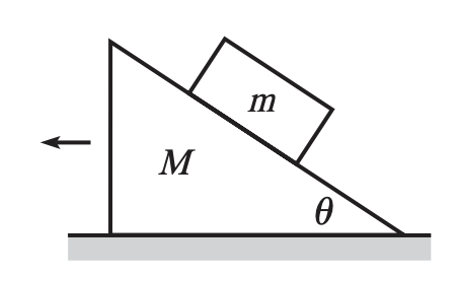
\includegraphics[width=0.6\textwidth]{P4.png}
    \label{P4}
\end{figure}

\subsection*{Solution}
Let \(v\) be the velocity of the wedge to the right, and let the block slide a distance \(d\) down the incline. Let \(u\) be the speed of the block relative to the wedge along the incline.

Choose \(x\) horizontal and \(y\) vertical. The block velocity is
\[
v_{bx}=v-u\cos\theta,
\qquad
v_{by}=-u\sin\theta.
\]

The horizontal momentum is conserved:
\[
Mv+m(v-u\cos\theta)=0.
\]

Thus
\[
(M+m)v=mu\cos\theta,
\]
so
\[
v=\frac{m u\cos\theta}{M+m}.
\]

The block descends vertically by
\[
h=d\sin\theta.
\]

Conservation of energy gives
\[
mgd\sin\theta
=
\frac12 Mv^2
+
\frac12 m\left[(v-u\cos\theta)^2+u^2\sin^2\theta\right].
\]

Simplify the block kinetic energy:
\[
(v-u\cos\theta)^2+u^2\sin^2\theta
=
v^2-2vu\cos\theta+u^2.
\]

So
\[
mgd\sin\theta
=
\frac12(M+m)v^2
-
mvu\cos\theta
+
\frac12 m u^2.
\]

Using
\[
v=\frac{m u\cos\theta}{M+m},
\]
we obtain
\[
mgd\sin\theta
=
\frac12 m u^2
-
\frac12\frac{m^2u^2\cos^2\theta}{M+m}.
\]

Therefore
\[
mgd\sin\theta
=
\frac12 m u^2
\left(
1-\frac{m\cos^2\theta}{M+m}
\right).
\]

Hence
\[
u^2
=
\frac{2gd\sin\theta(M+m)}
{M+m-m\cos^2\theta}.
\]

The wedge speed is
\[
v=\frac{m u\cos\theta}{M+m}.
\]

Therefore
\[
\boxed{
v
=
\frac{m\cos\theta}{M+m}
\sqrt{
\frac{2gd\sin\theta(M+m)}
{M+m-m\cos^2\theta}
}.
}
\]

Equivalently,
\[
\boxed{
v^2
=
\frac{2m^2gd\sin\theta\cos^2\theta}
{(M+m)(M+m-m\cos^2\theta)}.
}
\]


\newpage
\section*{Problem 5 [$5 + 5$ points]}
A particle of mass $m$ moves in one dimension with Lagrangian
\begin{equation*}
    L(q,\dot{q})=\frac{1}{2}m\dot{q}^2+A(q)\,\dot{q}-V(q),
\end{equation*}
where $A(q)$ and $V(q)$ are given functions.

\begin{enumerate}
\item[(1)] Find the canonical momentum $p$ conjugate to $q$.

\item[(2)] Find the Hamiltonian $H(q,p)$.
\end{enumerate}

\subsection*{Solution}
The Lagrangian is
\[
L(q,\dot q)
=
\frac12 m\dot q^2
+
A(q)\dot q
-
V(q).
\]

\begin{enumerate}
\item[(1)] The canonical momentum is
\[
p=\frac{\partial L}{\partial \dot q}
=
m\dot q+A(q).
\]

Thus
\[
\boxed{
p=m\dot q+A(q).
}
\]

\item[(2)] Solve for \(\dot q\):
\[
\dot q=\frac{p-A(q)}{m}.
\]

The Hamiltonian is
\[
H=p\dot q-L.
\]

Substituting,
\[
H
=
p\dot q
-
\left[
\frac12 m\dot q^2
+
A(q)\dot q
-
V(q)
\right].
\]

Thus
\[
H
=
[p-A(q)]\dot q
-
\frac12 m\dot q^2
+
V(q).
\]

Since \(p-A(q)=m\dot q\),
\[
H
=
m\dot q^2
-
\frac12 m\dot q^2
+
V(q)
=
\frac12 m\dot q^2+V(q).
\]

Therefore
\[
\boxed{
H(q,p)=\frac{[p-A(q)]^2}{2m}+V(q).
}
\]

\end{enumerate}


\newpage
\section*{Problem 6 [$6 + 10$ points]}
\begin{enumerate}
\item[(1)]  What are the conditions on the ``small'' constants $a$, $b$, $c$, $d$, $e$, and $f$ in order that
\begin{equation*}
    q= Q+ aQ^2+2bQP + cP^2
\end{equation*}
\begin{equation*}
   p=P+dQ^2+2eQP+fP^2
\end{equation*}
be a canonical transformation to \textbf{first order} in small quantities?

\item[(2)] The Hamiltonian for a slightly anharmonic oscillator is
\begin{equation*}
   H=\frac{p^2}{2m} + \frac{1}{2}m\omega^2q^2 + \beta q p^2
\end{equation*}
where $\beta$ is ``small''. Perform a canonical transformation of the type given in (1) and adjust the constants so that the new Hamiltonian does not contain any cubic terms to first order in $\beta$, thus
\begin{equation*}
   H'=\frac{P^2}{2m} + \frac{1}{2}m\omega^2Q^2 + \mathcal{O}(\beta^2).
\end{equation*}
Write down the transformation rules between $(q, p)$ and $(Q, P)$.
\end{enumerate}

\subsection*{Solution}
\begin{enumerate}
\item[(1)] We have
\[
q=Q+aQ^2+2bQP+cP^2,
\]
\[
p=P+dQ^2+2eQP+fP^2.
\]

For a one-dimensional canonical transformation,
\[
\{q,p\}_{Q,P}=1.
\]

Compute
\[
\frac{\partial q}{\partial Q}
=
1+2aQ+2bP,
\qquad
\frac{\partial q}{\partial P}
=
2bQ+2cP,
\]
and
\[
\frac{\partial p}{\partial Q}
=
2dQ+2eP,
\qquad
\frac{\partial p}{\partial P}
=
1+2eQ+2fP.
\]

Thus
\[
\{q,p\}
=
\frac{\partial q}{\partial Q}\frac{\partial p}{\partial P}
-
\frac{\partial q}{\partial P}\frac{\partial p}{\partial Q}.
\]

To first order in the small constants, the second product is second order and can be neglected. Hence
\[
\{q,p\}
=
(1+2aQ+2bP)(1+2eQ+2fP)
+
\mathcal O(2).
\]

So
\[
\{q,p\}
=
1+2(a+e)Q+2(b+f)P+\mathcal O(2).
\]

For the transformation to be canonical to first order,
\[
\boxed{
a+e=0,
\qquad
b+f=0.
}
\]

Equivalently,
\[
\boxed{
e=-a,
\qquad
f=-b.
}
\]

There is no first-order condition on \(c\) or \(d\).

\item[(2)] The Hamiltonian is
\[
H=
\frac{p^2}{2m}
+
\frac12 m\omega^2q^2
+
\beta q p^2.
\]

We use the transformation
\[
q=Q+aQ^2+2bQP+cP^2,
\]
\[
p=P+dQ^2+2eQP+fP^2,
\]
with
\[
e=-a,
\qquad
f=-b.
\]

To first order in the small constants, write
\[
q=Q+\delta q,
\qquad
p=P+\delta p,
\]
where
\[
\delta q=aQ^2+2bQP+cP^2,
\]
\[
\delta p=dQ^2-2aQP-bP^2.
\]

The harmonic part becomes
\[
H_0
=
\frac{P^2}{2m}
+
\frac12 m\omega^2Q^2
+
\frac{P}{m}\delta p
+
m\omega^2Q\delta q.
\]

The cubic perturbation may be evaluated using zeroth-order variables:
\[
\beta q p^2
=
\beta QP^2+\mathcal O(\beta^2).
\]

The cubic terms in the transformed Hamiltonian are therefore
\[
H_3
=
\frac{P}{m}
\left(dQ^2-2aQP-bP^2\right)
+
m\omega^2Q
\left(aQ^2+2bQP+cP^2\right)
+
\beta QP^2.
\]

Collecting powers:
\[
H_3
=
m\omega^2 a Q^3
+
\left(\frac{d}{m}+2m\omega^2 b\right)Q^2P
+
\left(-\frac{2a}{m}+m\omega^2 c+\beta\right)QP^2
-
\frac{b}{m}P^3.
\]

We require all cubic coefficients to vanish:
\[
m\omega^2a=0,
\]
\[
\frac{d}{m}+2m\omega^2b=0,
\]
\[
-\frac{2a}{m}+m\omega^2c+\beta=0,
\]
\[
-\frac{b}{m}=0.
\]

Therefore
\[
a=0,
\qquad
b=0,
\qquad
d=0,
\qquad
c=-\frac{\beta}{m\omega^2}.
\]

Since
\[
e=-a,
\qquad
f=-b,
\]
we also have
\[
e=0,
\qquad
f=0.
\]

Thus the required transformation is
\[
\boxed{
q=Q-\frac{\beta}{m\omega^2}P^2,
\qquad
p=P.
}
\]

To first order in \(\beta\), the inverse transformation is
\[
\boxed{
Q=q+\frac{\beta}{m\omega^2}p^2,
\qquad
P=p.
}
\]

With this choice,
\[
\boxed{
H'
=
\frac{P^2}{2m}
+
\frac12 m\omega^2Q^2
+
\mathcal O(\beta^2).
}
\]

\end{enumerate}


\newpage
\section*{Problem 7 [$12$ points]}
A mass $m$ is attached to one end of a massless spring of natural length $l_0$ and spring constant $k$. The other end of the spring is attached to a pivot point that oscillates vertically according to $Y(t)=A\cos(\Omega t).$ The mass moves in a vertical plane. Let $r$ be the instantaneous length of the spring, and let $\theta$ be the angle the spring makes with the downward vertical direction. This is a spring pendulum whose pivot oscillates vertically.  Construct the Lagrangian for the system and derive the equations of motion for $r(t)$ and $\theta(t)$.

\begin{figure}[h]
    \centering
    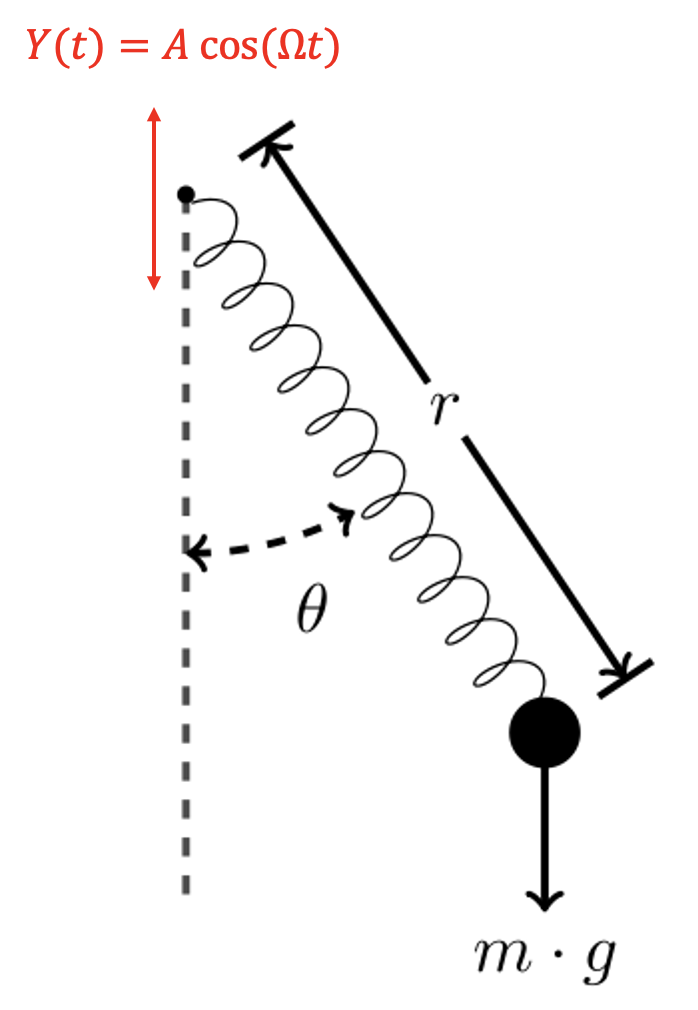
\includegraphics[width=0.4\textwidth]{P7.png}
    \label{P4}
\end{figure}

\subsection*{Solution}
Let the pivot have vertical coordinate
\[
Y(t)=A\cos(\Omega t).
\]

Choose \(y\) upward and \(x\) horizontal. Since \(\theta\) is measured from the downward vertical,
\[
x=r\sin\theta,
\]
\[
y=Y(t)-r\cos\theta.
\]

Then
\[
\dot x=\dot r\sin\theta+r\dot\theta\cos\theta,
\]
\[
\dot y=\dot Y-\dot r\cos\theta+r\dot\theta\sin\theta.
\]

Thus
\[
v^2=\dot x^2+\dot y^2.
\]

Expanding,
\[
v^2
=
\dot r^2+r^2\dot\theta^2+\dot Y^2
-2\dot Y\dot r\cos\theta
+
2\dot Y r\dot\theta\sin\theta.
\]

Therefore
\[
T
=
\frac12 m
\left(
\dot r^2+r^2\dot\theta^2+\dot Y^2
-2\dot Y\dot r\cos\theta
+
2\dot Y r\dot\theta\sin\theta
\right).
\]

The potential energy is
\[
V
=
\frac12 k(r-l_0)^2
+
mg\left(Y-r\cos\theta\right).
\]

Thus the Lagrangian is
\[
\boxed{
L
=
\frac12 m
\left(
\dot r^2+r^2\dot\theta^2+\dot Y^2
-2\dot Y\dot r\cos\theta
+
2\dot Y r\dot\theta\sin\theta
\right)
-
\frac12 k(r-l_0)^2
-
mg\left(Y-r\cos\theta\right).
}
\]

Terms depending only on time may be dropped. An equivalent Lagrangian is
\[
\boxed{
L
=
\frac12 m
\left(
\dot r^2+r^2\dot\theta^2
-2\dot Y\dot r\cos\theta
+
2\dot Y r\dot\theta\sin\theta
\right)
+
mgr\cos\theta
-
\frac12 k(r-l_0)^2.
}
\]

Using the Euler--Lagrange equations, or equivalently working in the accelerating frame of the pivot, the equations of motion are
\[
\boxed{
\ddot r
=
r\dot\theta^2
+
\left(g+\ddot Y\right)\cos\theta
-
\frac{k}{m}(r-l_0).
}
\]

and
\[
\boxed{
r\ddot\theta
+
2\dot r\dot\theta
+
\left(g+\ddot Y\right)\sin\theta
=0.
}
\]

Since
\[
Y(t)=A\cos(\Omega t),
\]
we have
\[
\ddot Y(t)=-A\Omega^2\cos(\Omega t).
\]

Therefore the equations may also be written as
\[
\boxed{
\ddot r
=
r\dot\theta^2
+
\left[g-A\Omega^2\cos(\Omega t)\right]\cos\theta
-
\frac{k}{m}(r-l_0),
}
\]
\[
\boxed{
r\ddot\theta
+
2\dot r\dot\theta
+
\left[g-A\Omega^2\cos(\Omega t)\right]\sin\theta
=0.
}
\]


\newpage
\section*{Problem 8 [$12$ points]}
A satellite of mass $m$ carrying a crew is initially in a stable circular orbit (Orbit 1) of radius $R_1$ around a central body of mass $M$. The crew wishes to transfer the satellite to a larger circular orbit (Orbit 3) with a radius of $R_3 = 2R_1$. To achieve this, they perform a maneuver involving two successive impulsive boosts.
First, the satellite performs an initial boost that increases its velocity instantaneously, placing it onto an elliptical transfer orbit (denoted as Orbit 2). This transfer orbit has its perigee at radius $R_1$ (the radius of the initial circular orbit) and its apogee at $R_3 = 2R_1$.
Next, upon reaching the apogee of the transfer orbit (point $P'$), the satellite performs a second instantaneous velocity change. This second boost increases the satellite's speed such that it transitions into a final circular orbit of radius $2R_1$.
\begin{enumerate}
    \item[(1)] Determine the thrust factor $\lambda$ required for the first boost, defined as the ratio of the speed after the boost to the speed before the boost ($\lambda = v_{p} / v_1$).
    \item[(2)] Determine the thrust factor $\lambda'$ required for the second boost, defined as the ratio of the speed after the boost to the speed before the boost ($\lambda' = v_3 / v_{p'}$).
\end{enumerate}

\textbf{Hint:} The orbit of a satellite is given by
$r(\phi) = \frac{c}{1 + \epsilon \cos \phi}$.
$\epsilon$ is the eccentricity of the orbit; $c = \frac{L^2}{GMm^2}$, where $L$ is the satellite's angular momentum.

\begin{figure}[h]
    \centering
    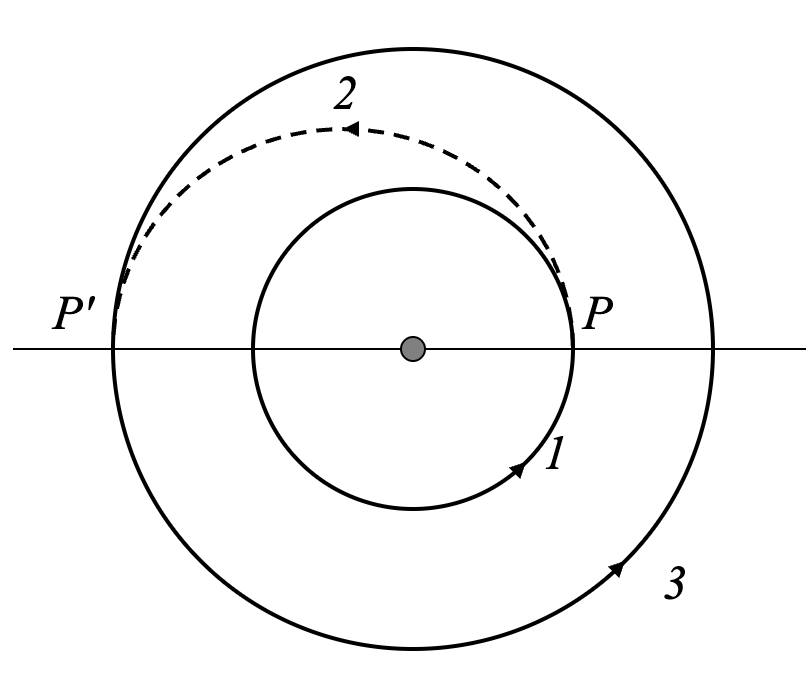
\includegraphics[width=0.3\textwidth]{transfer.png}
    \label{P7}
\end{figure}

\subsection*{Solution}
Let
\[
\mu=GM.
\]

The initial circular orbit has radius
\[
R_1.
\]

Thus the initial circular speed is
\[
v_1=\sqrt{\frac{\mu}{R_1}}.
\]

The final circular orbit has radius
\[
R_3=2R_1.
\]

The transfer orbit is an ellipse with perigee
\[
r_p=R_1
\]
and apogee
\[
r_a=2R_1.
\]

The semi-major axis is
\[
a=\frac{r_p+r_a}{2}
=
\frac{R_1+2R_1}{2}
=
\frac32 R_1.
\]

For an elliptic orbit, the vis-viva equation is
\[
v^2=\mu\left(\frac{2}{r}-\frac{1}{a}\right).
\]

At perigee,
\[
v_p^2
=
\mu\left(
\frac{2}{R_1}
-
\frac{1}{(3/2)R_1}
\right)
=
\mu\left(
\frac{2}{R_1}
-
\frac{2}{3R_1}
\right)
=
\frac{4\mu}{3R_1}.
\]

Thus
\[
v_p=\sqrt{\frac{4\mu}{3R_1}}.
\]

Therefore
\[
\lambda
=
\frac{v_p}{v_1}
=
\frac{\sqrt{4\mu/(3R_1)}}{\sqrt{\mu/R_1}}
=
\sqrt{\frac43}.
\]

Hence
\[
\boxed{
\lambda=\sqrt{\frac43}.
}
\]

At apogee,
\[
r=2R_1.
\]

The transfer-orbit speed at apogee is
\[
v_{p'}^2
=
\mu
\left(
\frac{2}{2R_1}
-
\frac{1}{(3/2)R_1}
\right)
=
\mu
\left(
\frac{1}{R_1}
-
\frac{2}{3R_1}
\right)
=
\frac{\mu}{3R_1}.
\]

Thus
\[
v_{p'}=\sqrt{\frac{\mu}{3R_1}}.
\]

The circular speed in the final orbit is
\[
v_3=\sqrt{\frac{\mu}{2R_1}}.
\]

Therefore
\[
\lambda'
=
\frac{v_3}{v_{p'}}
=
\frac{\sqrt{\mu/(2R_1)}}{\sqrt{\mu/(3R_1)}}
=
\sqrt{\frac32}.
\]

Thus
\[
\boxed{
\lambda'=\sqrt{\frac32}.
}
\]

Numerically,
\[
\lambda\approx 1.155,
\qquad
\lambda'\approx 1.225.
\]


\newpage
\section*{Problem 9 [$10$ points]}
The Lagrangian for a particle of mass $m$ and charge $e$ moving in a uniform magnetic field which points in the $z$-direction is
\[
L = \frac{1}{2}m({\dot{x}^2} + {\dot{y}^2}  + {\dot{z}^2} ) + (eB/2c)(x\dot{y} - y\dot{x})
\]
Show that the system is invariant under spatial displacement along $x$ and find the associated constants of the motion.

\subsection*{Solution}
The Lagrangian is
\[
L
=
\frac12 m(\dot x^2+\dot y^2+\dot z^2)
+
\frac{eB}{2c}(x\dot y-y\dot x).
\]

Define
\[
\alpha=\frac{eB}{2c}.
\]

Then
\[
L
=
\frac12 m(\dot x^2+\dot y^2+\dot z^2)
+
\alpha(x\dot y-y\dot x).
\]

The canonical momentum conjugate to \(x\) is
\[
p_x=\frac{\partial L}{\partial \dot x}
=
m\dot x-\alpha y.
\]

Consider an infinitesimal spatial displacement along \(x\):
\[
x\to x+\epsilon,
\qquad
y\to y,
\qquad
z\to z.
\]

Thus
\[
\delta x=\epsilon,
\qquad
\delta y=0,
\qquad
\delta z=0.
\]

The velocities do not change:
\[
\delta\dot x=0,
\qquad
\delta\dot y=0,
\qquad
\delta\dot z=0.
\]

The change in the Lagrangian is
\[
\delta L
=
\alpha\epsilon \dot y.
\]

This is a total time derivative:
\[
\delta L
=
\frac{d}{dt}(\alpha\epsilon y).
\]

Therefore the action is invariant under displacement along \(x\), even though the Lagrangian changes by a total derivative.

By Noether's theorem, if
\[
\delta L=\frac{dF}{dt},
\]
then the conserved quantity is
\[
Q=\sum_i p_i\delta q_i-F.
\]

Here
\[
F=\alpha\epsilon y.
\]

Therefore
\[
Q
=
p_x\epsilon-\alpha\epsilon y.
\]

Dividing by \(\epsilon\),
\[
Q_x=p_x-\alpha y.
\]

Using
\[
p_x=m\dot x-\alpha y,
\]
we find
\[
Q_x
=
m\dot x-2\alpha y.
\]

Since
\[
2\alpha=\frac{eB}{c},
\]
the conserved quantity is
\[
\boxed{
Q_x
=
m\dot x-\frac{eB}{c}y.
}
\]

Equivalently,
\[
\boxed{
Q_x=p_x-\frac{eB}{2c}y.
}
\]

One may check directly using the equations of motion. The Euler--Lagrange equation for \(x\) gives
\[
m\ddot x=\frac{eB}{c}\dot y.
\]

Therefore
\[
\frac{d}{dt}
\left(
m\dot x-\frac{eB}{c}y
\right)
=
m\ddot x-\frac{eB}{c}\dot y
=0.
\]

Thus \(Q_x\) is conserved.


\newpage
\section*{Bonus Problem [$6$ points]}
The Hamiltonian for a simple harmonic oscillator is
\[
H=\frac{p^2}{2m}+\frac{1}{2}m\omega^2 x^2.
\]
Introduce the complex quantities
\[
a=\sqrt{\frac{m\omega}{2}}\left(x+\frac{i p}{m\omega}\right) \quad \text{and} \quad a^*=\sqrt{\frac{m\omega}{2}}\left(x-\frac{i p}{m\omega}\right).
\]

\begin{enumerate}
    \item[(a)] Express $H$ in terms of $a$ and $a^*$.

    \item[(b)] Evaluate the Poisson brackets $[a,a^*]$, $[a,H]$, and $[a^*,H]$.
\end{enumerate}

\subsection*{Solution}
The Hamiltonian is
\[
H=\frac{p^2}{2m}+\frac12 m\omega^2x^2.
\]

The complex variables are
\[
a=
\sqrt{\frac{m\omega}{2}}
\left(
x+\frac{ip}{m\omega}
\right),
\qquad
a^*
=
\sqrt{\frac{m\omega}{2}}
\left(
x-\frac{ip}{m\omega}
\right).
\]

\begin{enumerate}
\item[(a)] Compute
\[
aa^*
=
\frac{m\omega}{2}
\left(
x+\frac{ip}{m\omega}
\right)
\left(
x-\frac{ip}{m\omega}
\right).
\]

Thus
\[
aa^*
=
\frac{m\omega}{2}
\left(
x^2+\frac{p^2}{m^2\omega^2}
\right).
\]

Therefore
\[
\omega aa^*
=
\frac12 m\omega^2x^2+\frac{p^2}{2m}.
\]

Hence
\[
\boxed{
H=\omega aa^*.
}
\]

\item[(b)] The Poisson bracket is
\[
[A,B]
=
\frac{\partial A}{\partial x}\frac{\partial B}{\partial p}
-
\frac{\partial A}{\partial p}\frac{\partial B}{\partial x}.
\]

We have
\[
\frac{\partial a}{\partial x}
=
\sqrt{\frac{m\omega}{2}},
\qquad
\frac{\partial a}{\partial p}
=
i\sqrt{\frac{m\omega}{2}}\frac{1}{m\omega}
=
\frac{i}{\sqrt{2m\omega}}.
\]

Also,
\[
\frac{\partial a^*}{\partial x}
=
\sqrt{\frac{m\omega}{2}},
\qquad
\frac{\partial a^*}{\partial p}
=
-\frac{i}{\sqrt{2m\omega}}.
\]

Therefore
\[
[a,a^*]
=
\sqrt{\frac{m\omega}{2}}
\left(
-\frac{i}{\sqrt{2m\omega}}
\right)
-
\frac{i}{\sqrt{2m\omega}}
\sqrt{\frac{m\omega}{2}}.
\]

Thus
\[
\boxed{
[a,a^*]=-i.
}
\]

Using
\[
H=\omega aa^*,
\]
we get
\[
[a,H]
=
\omega[a,aa^*]
=
\omega\left([a,a]a^*+a[a,a^*]\right).
\]

Since
\[
[a,a]=0,
\qquad
[a,a^*]=-i,
\]
we find
\[
\boxed{
[a,H]=-i\omega a.
}
\]

Similarly,
\[
[a^*,H]
=
\omega[a^*,aa^*]
=
\omega\left([a^*,a]a^*+a[a^*,a^*]\right).
\]

Since
\[
[a^*,a]=i,
\qquad
[a^*,a^*]=0,
\]
we get
\[
\boxed{
[a^*,H]=i\omega a^*.
}
\]

\end{enumerate}


\end{document}